% !TEX program = lualatex
% Generated by new_homework.sh — Math 104 Homework 4
\documentclass[11pt]{article}

\usepackage{fontspec}
\usepackage{microtype}
\usepackage{mathtools,amssymb,amsfonts,amsthm,bm}
\usepackage{enumitem}
\usepackage{booktabs,array,xcolor}
\usepackage{geometry,fancyhdr,setspace}
\usepackage{pdfpages}
\usepackage[hidelinks]{hyperref}
\usepackage[nameinlink,noabbrev]{cleveref}

% ---------- Page and paragraph rhythm (matches lecture/solutions templates) ----------
\geometry{margin=1in,headheight=15pt}
\setstretch{1.12}
\setlength{\parindent}{0pt}
\setlength{\parskip}{0.55em plus 0.12em minus 0.08em}
\setlength{\abovedisplayskip}{0.8em plus 0.2em minus 0.1em}
\setlength{\belowdisplayskip}{0.8em plus 0.2em minus 0.1em}
\allowdisplaybreaks[3]
\setlist{leftmargin=*,topsep=0.35em,itemsep=0.15em,parsep=0pt}

% ---------- Metadata ----------
\newcommand{\studentname}{Keshav Ramamurthy}
\newcommand{\coursename}{Math 104}
\newcommand{\courselongname}{Real Analysis}
\newcommand{\assignment}{Homework 4}
\newcommand{\term}{Fall 2026}

% ---------- Core notation (same as ~/.config/nvim/textemplate.tex) ----------
\newcommand{\N}{\mathbb{N}}
\newcommand{\Z}{\mathbb{Z}}
\newcommand{\Q}{\mathbb{Q}}
\newcommand{\R}{\mathbb{R}}
\newcommand{\C}{\mathbb{C}}
\newcommand{\F}{\mathbb{F}}
\newcommand{\K}{\mathbb{K}}
\newcommand{\E}{\mathbb{E}}
\newcommand{\Prob}{\mathbb{P}}
\newcommand{\1}{\mathbf{1}}
\newcommand{\eps}{\varepsilon}
\newcommand{\dd}{\,\mathrm{d}}
\newcommand{\abs}[1]{\left\lvert#1\right\rvert}
\newcommand{\norm}[1]{\left\lVert#1\right\rVert}
\newcommand{\ip}[2]{\left\langle#1,#2\right\rangle}
\newcommand{\set}[1]{\left\{#1\right\}}
\newcommand{\ceil}[1]{\left\lceil#1\right\rceil}
\newcommand{\floor}[1]{\left\lfloor#1\right\rfloor}
\newcommand{\given}{\,\middle\vert\,}
\newcommand{\indep}{\perp\!\!\!\perp}
\newcommand{\wh}[1]{\widehat{#1}}
\newcommand{\deriv}[2]{\frac{\mathrm{d}#1}{\mathrm{d}#2}}
\newcommand{\pderiv}[2]{\frac{\partial#1}{\partial#2}}
\newcommand{\lto}{\longrightarrow}
\newcommand{\st}{\text{ such that }}
\DeclareMathOperator{\Aut}{Aut}
\DeclareMathOperator{\End}{End}
\DeclareMathOperator{\Gal}{Gal}
\DeclareMathOperator{\Hom}{Hom}
\DeclareMathOperator{\Ker}{ker}
\DeclareMathOperator{\im}{im}
\DeclareMathOperator{\rank}{rank}
\DeclareMathOperator{\nullity}{nullity}
\DeclareMathOperator{\Span}{span}
\DeclareMathOperator{\tr}{tr}
\DeclareMathOperator{\diag}{diag}
\DeclareMathOperator{\spec}{spec}
\DeclareMathOperator{\ord}{ord}
\DeclareMathOperator{\supp}{supp}
\DeclareMathOperator{\diam}{diam}
\DeclareMathOperator{\Var}{Var}
\DeclareMathOperator{\Cov}{Cov}
\DeclareMathOperator*{\argmin}{arg\,min}
\DeclareMathOperator*{\argmax}{arg\,max}

% ---------- Statement environments ----------
\newtheorem{problem}{Problem}
\newtheorem{theorem}{Theorem}
\newtheorem{lemma}{Lemma}
\newtheorem{proposition}{Proposition}
\newtheorem{corollary}{Corollary}
\theoremstyle{definition}
\newtheorem{definition}{Definition}
\newtheorem{example}{Example}
\newtheorem{remark}{Remark}

% ---------- Solution machinery (matches solutions.tex / textemplate.tex) ----------
\newenvironment{solution}{\begin{proof}[Solution]}{\end{proof}}
\newenvironment{answer}{\begin{proof}[Answer]}{\end{proof}}
\renewcommand{\qedsymbol}{\(\square\)}
\newcommand{\exercise}[1]{%
  \par\goodbreak\medskip\noindent\textbf{Exercise #1}\par\nopagebreak\smallskip\nopagebreak}
\newcommand{\exref}[1]{\textsf{\textbf{Exercise~#1}}}
\newenvironment{claim}{\par\smallskip\noindent\textit{Claim.}\ }{\par\smallskip}
\newenvironment{idea}{\par\smallskip\noindent\textit{Idea.}\ }{\par\smallskip}
\newenvironment{proofsketch}{\par\smallskip\noindent\textit{Proof sketch.}\ }{\par\smallskip}

% ---------- Header ----------
\pagestyle{fancy}
\fancyhf{}
\fancyhead[L]{\coursename}
\fancyhead[C]{\assignment\ — my solutions}
\fancyhead[R]{\studentname}
\fancyfoot[C]{\thepage}

\begin{document}

% ---------- Title ----------
\begin{center}
  {\Large\sffamily\bfseries \coursename\ -- \courselongname}\par\vspace{3pt}
  {\sffamily \assignment\ — my solutions}\par\vspace{3pt}
  {\small\sffamily \term\quad\textbullet\quad \studentname}
\end{center}
\medskip
\hrule
\bigskip

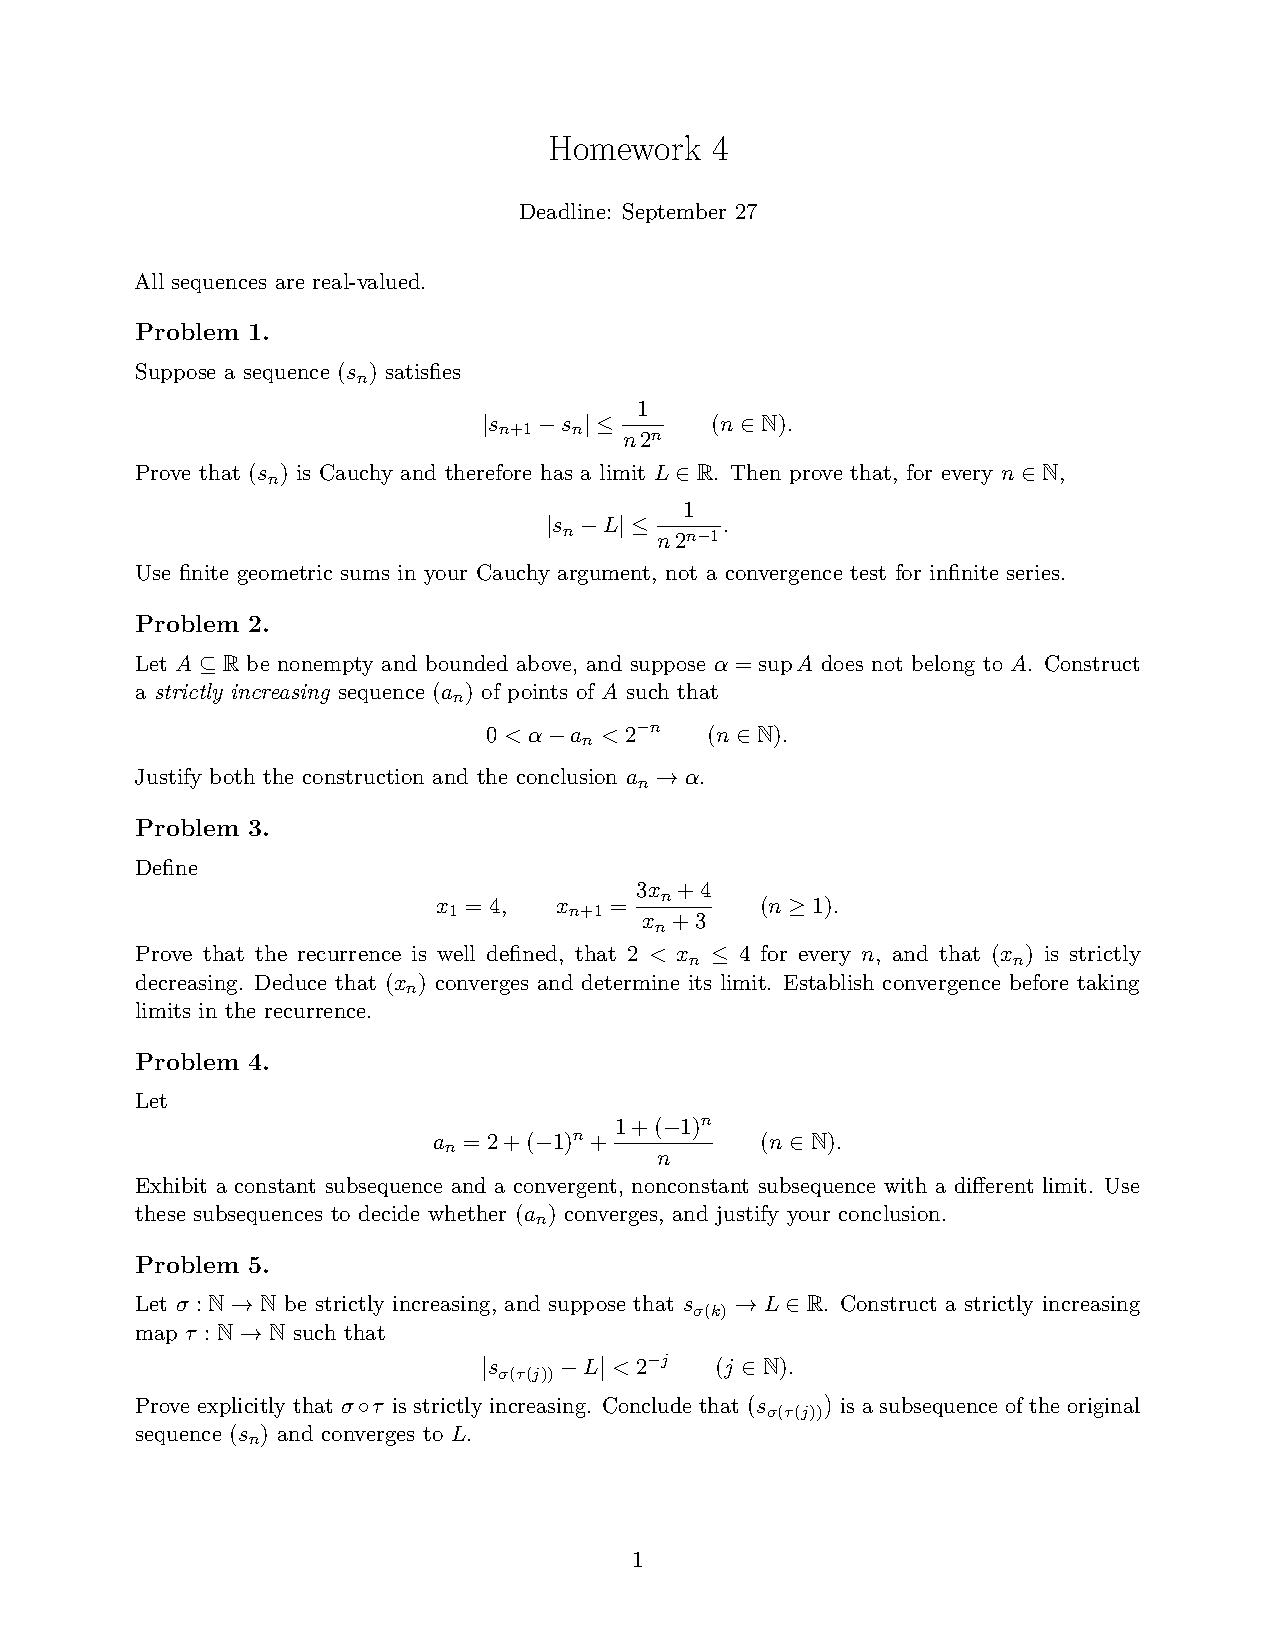
\includepdf[pages=-,pagecommand={\thispagestyle{empty}}]{HW4.pdf}
\clearpage

\section*{Solutions}
\subsubsection*{Problem 1}
\begin{solution}
We do this using triangle inequality.
For our scratch work, Let's bound \[|s_{m} - s_{n}| = |(s_m -s_{m-1}) + (s_{m-1} - s_{m-2}) + \cdots +
(s_{n+1} - s_{n})| \le \sum_{i=n}^{m-1}|s_{i+1}-s_i| \le \sum_{i=n}^{m-1} \frac{1}{i 2^i} \]
Since \(n \ge 1\), notice that \(\frac{1}{i 2^i}\le \frac{1}{2^i}\) and so we'll bound again,
\[\sum_{i=n}^{m-1}\frac{1}{i2^i} \le \sum_{i=n}^{m-1}\frac{1}{2^i} = \frac{1}{2^{n-1}} -
\frac{1}{2^{m-1}} < \frac{1}{2^{n-1}} < \epsilon\]
So if we rearrange, we can write
\(N = \max\left\{1,\left\lceil\log_{2}{\frac{1}{\epsilon}}\right\rceil + 2\right\}\), we have the Cauchy condition, namely
for an \(\epsilon > 0\), \[\forall n, m \ge N \implies |s_m - s_{n}| < \epsilon \]
and thus it has a limit \(L \in \mathbb{R}\).
\par Notice if \(\lim s_n = L\), then for each fixed \(n\), \(s_m \rightarrow L\), so
\[|s_n-L|=\lim_{m\rightarrow \infty} |s_n - s_m|.\]
\par To do this, we'll use the same triangle inequality idea
\[|s_n - s_m| \le \sum_{i=n}^{m-1} |s_{i+1}-s_i|\le\sum_{i=n}^{m-1} \frac{1}{i2^i}
\le \frac{1}{n}\sum_{i=n}^{m-1}\frac{1}{2^{i}}
\]
And this is really convenient as this sum is equal to
\[|s_m - s_n| \le
\frac{1}{n}\left(\frac{1}{2^{n-1}}-\frac{1}{2^{m-1}}\right).\]
Taking \(m\rightarrow\infty\), we get
\[|s_n-L| \le
\frac{1}{n}\left(\frac{1}{2^{n-1}}\right)
=\frac{1}{n2^{n-1}},\]
as desired.
% Write your proof, calculation, or argument here.
\end{solution}
\subsubsection*{Problem 2}
\begin{solution}
    To do this Let's first rearrange the condition to get \(\alpha > a_n > \alpha - 2^{-n}\)
% \par    Because a is increasing and bounded above, its limit exists.
\par We can construct it as follows. For \(a_1\) we have \(\alpha > a_1 > \alpha -
\frac{1}{2}\).
Then, for each \(i\ge 2\), we can find
\[\alpha > a_i > \max\{a_{i-1}, \alpha - 2^{-i}\}.\]
This is the construction, we claim that it's valid along the following lines.
Because \(a_{i-1}\in A\) and \(\alpha\notin A\), we have \(a_{i-1}<\alpha\), and also
\(\alpha-2^{-i}<\alpha\). Thus
\[\max\{a_{i-1},\alpha-2^{-i}\}<\alpha.\]
By the supremum property,
\[\exists a_i \in A \text{ such that } \alpha >  a_i > \max\{a_{i-1}, \alpha - 2^{-i}\},\]
and that justifies our construction. In particular, \(a_i>a_{i-1}\), so the sequence is
strictly increasing.
Because \(\alpha - 2^{-n} < a_n < \alpha \) and \(\alpha - 2^{-n} \rightarrow \alpha\), by
the squeeze theorem, \(a_n \rightarrow \alpha.\)
% Write your proof, calculation, or argument here.
\end{solution}
\subsubsection*{Problem 3}
\begin{solution}
    For this, let's first show \(x_n > 2\) by induction.
\par Our base case is \(x_1 = 4 > 2.\)
\par For the inductive step, suppose \(x_k > 2\) for an arbitrary \(k \in
\mathbb{Z}^{+}\). Since \(x_k+3>0\), the recurrence is well defined, and
\[
x_{k+1}-2
=
\frac{3x_k+4}{x_k+3}-2
=
\frac{x_k-2}{x_k+3}>0.
\]
Thus \(x_{k+1}>2\), so \(x_n>2\) for every \(n\).
\par Let's show \(x_{k + 1} < x_k.\)
\[
x_{k + 1} - x_k= \frac{3x_k + 4}{x_k + 3} - x_k
= \frac{4-x_k^2}{x_k+3}< 0,
\]
since \(x_k > 2\), so \(4-x_k^2 < 0\), while \(x_k + 3 > 0\).
Thus \((x_k)\) is strictly decreasing. Since \(x_1=4\), we have
\(2<x_n\le 4\) for every \(n\).
\par Because it is decreasing and bounded below, \(\lim_{k\rightarrow \infty} x_k = L\)
exists.
\par Notice similarly \(\lim_{k\rightarrow \infty} x_{k+1} = L\), so we write
\[
L = \lim_{k\rightarrow \infty} x_{k + 1}
= \lim_{k\rightarrow\infty} \frac{3x_k+4}{x_k+3}.
\]
Because \(x_k>2\) for every \(k\), we have \(L\ge 2\), so \(L+3\neq 0\). Therefore
\[
L = \frac{\lim (3x_k + 4)}{\lim (x_k + 3)} = \frac{3L + 4}{L + 3}.
\]
And solving this quadratic for \(L\) gets you
\[
L^2 + 3L = 3L + 4 \rightarrow L= \pm 2.
\]
Since \(L\ge 2\), we get \(L=2\).
% Write your proof, calculation, or argument here.
\end{solution}
\subsubsection*{Problem 4}
\begin{solution}
    If you examine the even elements, you see that
    \[\lim (a_{2k}) = \lim(2 + (-1)^{2k}) + \lim \frac{1+(-1)^{2k}}{2k} = 3 + 0 = 3\]
    However, if you examine the odd elements, you get
    \[\lim (a_{2k+1}) = \lim (2 + (-1)^{2k+1}) + \lim \frac{1+(-1)^{2k+1}}{2k+1} = 1 + 0 =
    1\]
    Notice the odd sequence is constant, because \(2 + (-1)^{2k+1} = 1\) and
    \(1+(-1)^{2k+1} = 0\), but the even sequence is convergent but non constant, because
    each term \(a_{2k} = 3 + \frac{1+(-1)^{2k}}{2k} = 3 + \frac{1}{k}\).
    If \((a_n)\) converged, then every subsequence of \((a_n)\) would converge to the same
    limit. Since the odd subsequence converges to \(1\) and the even subsequence converges
    to \(3\), \((a_n)\) does not converge.
% Write your proof, calculation, or argument here.
\end{solution}
\subsubsection*{Problem 5}
\begin{solution}
    We want a sequence such that $$|s_{\sigma(\tau(j))} - L| < 2^{-j}$$
    We can arrange this to
    $$L-2^{-j}<s_{\sigma(\tau(j))}<L+2^{-j}.$$
    Since $s_{\sigma(k)} \rightarrow L$, we can make a sequence $N_1, N_2, \cdots $
    where, for a specific \(j\), we can set $\epsilon = 2^{-j}$ and have
$$\exists  N_j \text{ such that } k \ge N_j \implies |s_{\sigma(k)} - L| < \epsilon = 2^{-j}$$
for each $j$ in $\mathbb{Z}^{+}$. To continue, set \(\tau(1)=N_1\), and for \(i\ge2\)
recursively construct
\[
\tau(i) = \max\{N_i, \tau(i-1) + 1\}.
\]
The $N_i$ ensures that $|s_{\sigma(\tau(i))}-L|<2^{-i}$ and the other term ensures that
\(\tau(i)>\tau(i-1)\), so \(\tau\) is strictly increasing.
We have that $\sigma$ is strictly increasing and since our constructed $\tau$ is
strictly increasing, we have that
\[
j > i \implies \tau(j) > \tau(i) \implies
\sigma(\tau(j)) > \sigma(\tau(i)),
\]
so \(\sigma\circ\tau\) is strictly increasing.
Thus, $(s_{\sigma(\tau(j))})$ is a subsequence of the original sequence $(s_n)$ and,
since
\[
0\le |s_{\sigma(\tau(j))}-L|<2^{-j}\rightarrow0,
\]
it converges to \(L\).
% Write your proof, calculation, or argument here.
\end{solution}

\end{document}
